\documentclass[1p]{elsarticle_modified}
%\bibliographystyle{elsarticle-num}

%\usepackage[colorlinks]{hyperref}
%\usepackage{abbrmath_seonhwa} %\Abb, \Ascr, \Acal ,\Abf, \Afrak
\usepackage{amsfonts}
\usepackage{amssymb}
\usepackage{amsmath}
\usepackage{amsthm}
\usepackage{scalefnt}
\usepackage{amsbsy}
\usepackage{kotex}
\usepackage{caption}
\usepackage{subfig}
\usepackage{color}
\usepackage{graphicx}
\usepackage{xcolor} %% white, black, red, green, blue, cyan, magenta, yellow
\usepackage{float}
\usepackage{setspace}
\usepackage{hyperref}

\usepackage{tikz}
\usetikzlibrary{arrows}

\usepackage{multirow}
\usepackage{array} % fixed length table
\usepackage{hhline}

%%%%%%%%%%%%%%%%%%%%%
\makeatletter
\renewcommand*\env@matrix[1][\arraystretch]{%
	\edef\arraystretch{#1}%
	\hskip -\arraycolsep
	\let\@ifnextchar\new@ifnextchar
	\array{*\c@MaxMatrixCols c}}
\makeatother %https://tex.stackexchange.com/questions/14071/how-can-i-increase-the-line-spacing-in-a-matrix
%%%%%%%%%%%%%%%

\usepackage[normalem]{ulem}

\newcommand{\msout}[1]{\ifmmode\text{\sout{\ensuremath{#1}}}\else\sout{#1}\fi}
%SOURCE: \msout is \stkout macro in https://tex.stackexchange.com/questions/20609/strikeout-in-math-mode

\newcommand{\cancel}[1]{
	\ifmmode
	{\color{red}\msout{#1}}
	\else
	{\color{red}\sout{#1}}
	\fi
}

\newcommand{\add}[1]{
	{\color{blue}\uwave{#1}}
}

\newcommand{\replace}[2]{
	\ifmmode
	{\color{red}\msout{#1}}{\color{blue}\uwave{#2}}
	\else
	{\color{red}\sout{#1}}{\color{blue}\uwave{#2}}
	\fi
}

\newcommand{\Sol}{\mathcal{S}} %segment
\newcommand{\D}{D} %diagram
\newcommand{\A}{\mathcal{A}} %arc


%%%%%%%%%%%%%%%%%%%%%%%%%%%%%5 test

\def\sl{\operatorname{\textup{SL}}(2,\Cbb)}
\def\psl{\operatorname{\textup{PSL}}(2,\Cbb)}
\def\quan{\mkern 1mu \triangleright \mkern 1mu}

\theoremstyle{definition}
\newtheorem{thm}{Theorem}[section]
\newtheorem{prop}[thm]{Proposition}
\newtheorem{lem}[thm]{Lemma}
\newtheorem{ques}[thm]{Question}
\newtheorem{cor}[thm]{Corollary}
\newtheorem{defn}[thm]{Definition}
\newtheorem{exam}[thm]{Example}
\newtheorem{rmk}[thm]{Remark}
\newtheorem{alg}[thm]{Algorithm}

\newcommand{\I}{\sqrt{-1}}
\begin{document}

%\begin{frontmatter}
%
%\title{Boundary parabolic representations of knots up to 8 crossings}
%
%%% Group authors per affiliation:
%\author{Yunhi Cho} 
%\address{Department of Mathematics, University of Seoul, Seoul, Korea}
%\ead{yhcho@uos.ac.kr}
%
%
%\author{Seonhwa Kim} %\fnref{s_kim}}
%\address{Center for Geometry and Physics, Institute for Basic Science, Pohang, 37673, Korea}
%\ead{ryeona17@ibs.re.kr}
%
%\author{Hyuk Kim}
%\address{Department of Mathematical Sciences, Seoul National University, Seoul 08826, Korea}
%\ead{hyukkim@snu.ac.kr}
%
%\author{Seokbeom Yoon}
%\address{Department of Mathematical Sciences, Seoul National University, Seoul, 08826,  Korea}
%\ead{sbyoon15@snu.ac.kr}
%
%\begin{abstract}
%We find all boundary parabolic representation of knots up to 8 crossings.
%
%\end{abstract}
%\begin{keyword}
%    \MSC[2010] 57M25 
%\end{keyword}
%
%\end{frontmatter}

%\linenumbers
%\tableofcontents
%
\newcommand\colored[1]{\textcolor{white}{\rule[-0.35ex]{0.8em}{1.4ex}}\kern-0.8em\color{red} #1}%
%\newcommand\colored[1]{\textcolor{white}{ #1}\kern-2.17ex	\textcolor{white}{ #1}\kern-1.81ex	\textcolor{white}{ #1}\kern-2.15ex\color{red}#1	}

{\Large $\underline{10_{114}~(K10a_{77})}$}

\setlength{\tabcolsep}{10pt}
\renewcommand{\arraystretch}{1.6}
\vspace{1cm}\begin{tabular}{m{100pt}>{\centering\arraybackslash}m{274pt}}
\multirow{5}{120pt}{
	\centering
	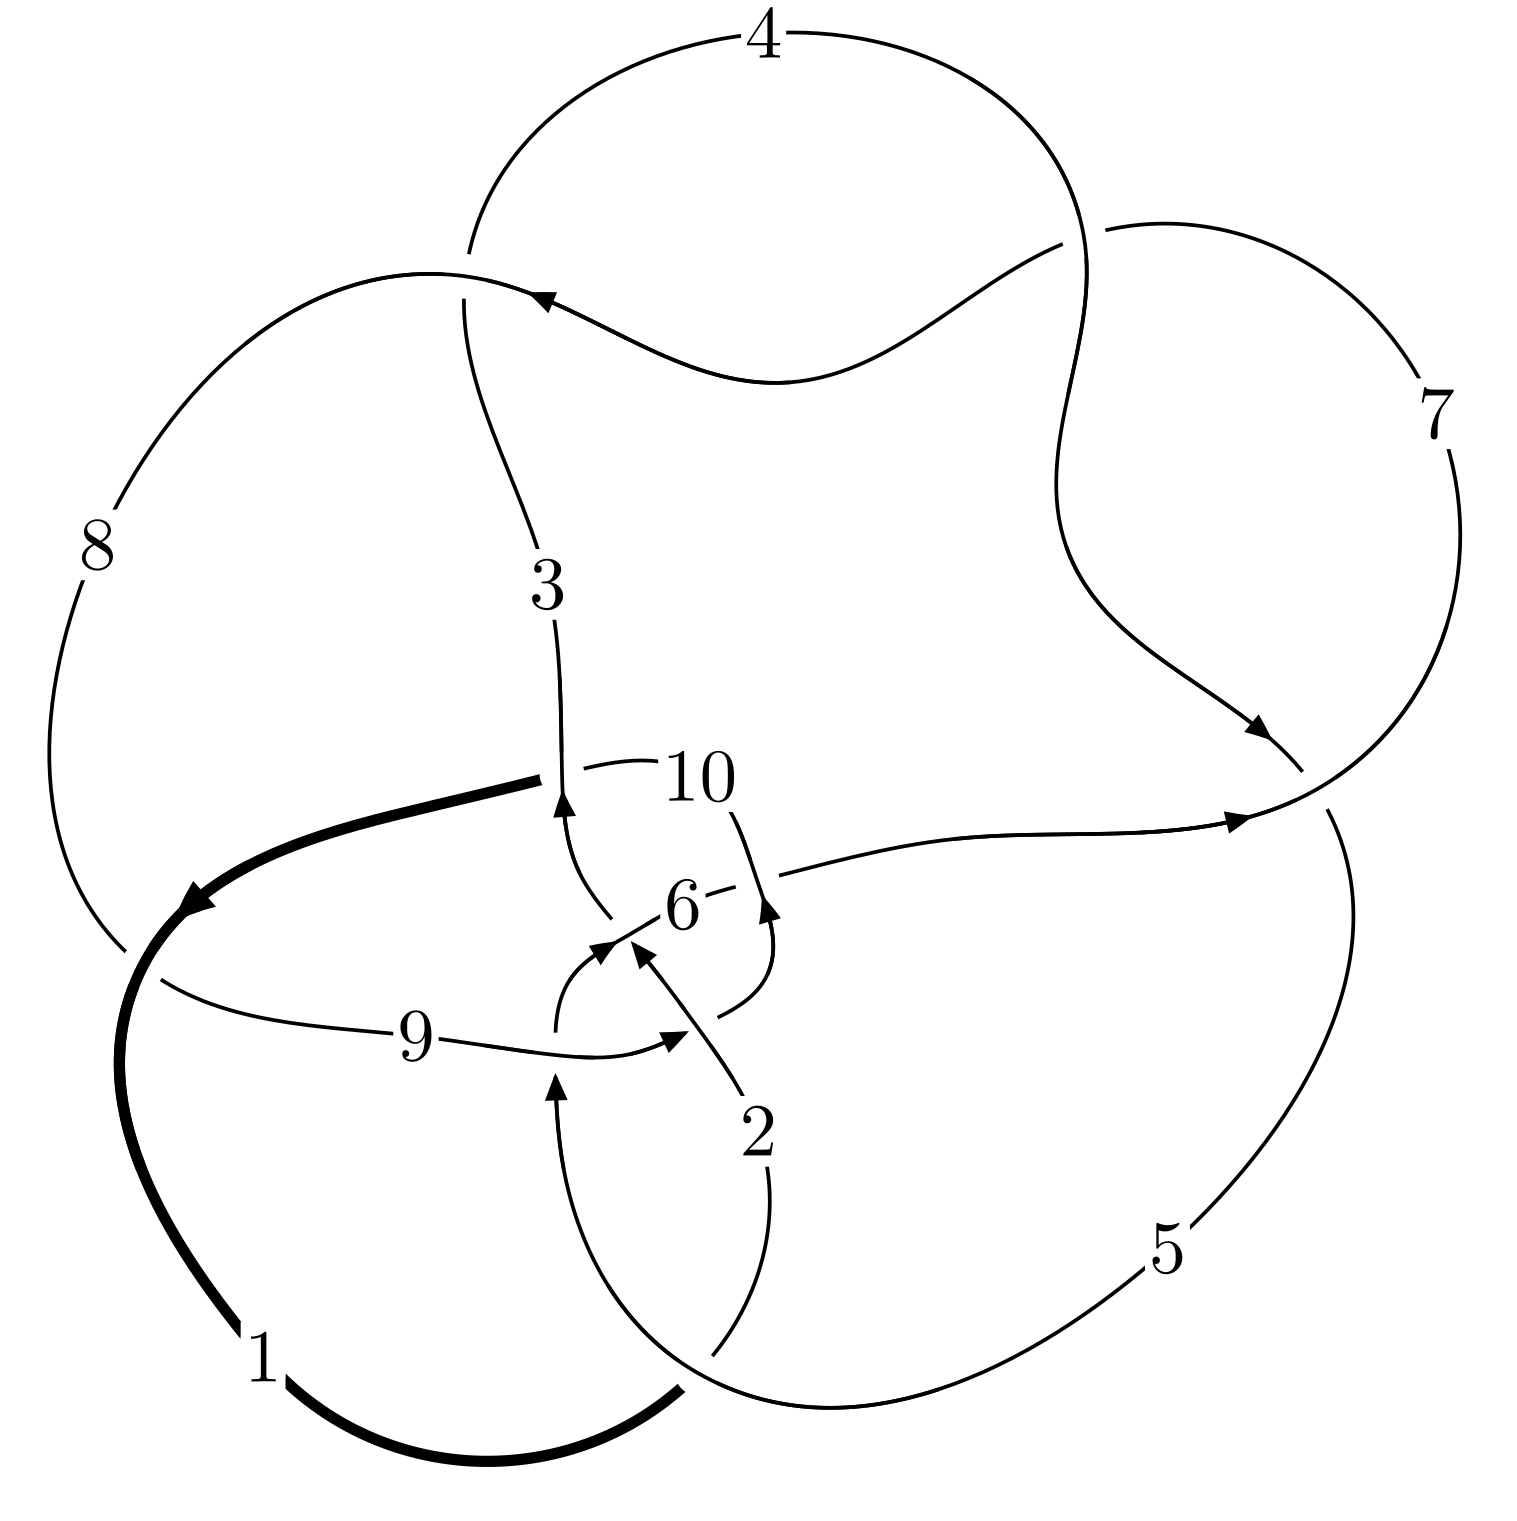
\includegraphics[width=112pt]{../../../GIT/diagram.site/Diagrams/png/198_10_114.png}\\
\ \ \ A knot diagram\footnotemark}&
\allowdisplaybreaks
\textbf{Linearized knot diagam} \\
\cline{2-2}
 &
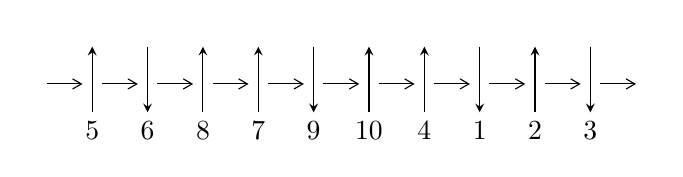
\begin{tikzpicture}[x=20pt, y=17pt]
	% nodes
	\node (C0) at (0, 0) {};
	\node (C1) at (1, 0) {};
	\node (C1U) at (1, +1) {};
	\node (C1D) at (1, -1) {5};

	\node (C2) at (2, 0) {};
	\node (C2U) at (2, +1) {};
	\node (C2D) at (2, -1) {6};

	\node (C3) at (3, 0) {};
	\node (C3U) at (3, +1) {};
	\node (C3D) at (3, -1) {8};

	\node (C4) at (4, 0) {};
	\node (C4U) at (4, +1) {};
	\node (C4D) at (4, -1) {7};

	\node (C5) at (5, 0) {};
	\node (C5U) at (5, +1) {};
	\node (C5D) at (5, -1) {9};

	\node (C6) at (6, 0) {};
	\node (C6U) at (6, +1) {};
	\node (C6D) at (6, -1) {10};

	\node (C7) at (7, 0) {};
	\node (C7U) at (7, +1) {};
	\node (C7D) at (7, -1) {4};

	\node (C8) at (8, 0) {};
	\node (C8U) at (8, +1) {};
	\node (C8D) at (8, -1) {1};

	\node (C9) at (9, 0) {};
	\node (C9U) at (9, +1) {};
	\node (C9D) at (9, -1) {2};

	\node (C10) at (10, 0) {};
	\node (C10U) at (10, +1) {};
	\node (C10D) at (10, -1) {3};
	\node (C11) at (11, 0) {};

	% arrows
	\draw[->,>={angle 60}]
	(C0) edge (C1) (C1) edge (C2) (C2) edge (C3) (C3) edge (C4) (C4) edge (C5) (C5) edge (C6) (C6) edge (C7) (C7) edge (C8) (C8) edge (C9) (C9) edge (C10) (C10) edge (C11) ;	\draw[->,>=stealth]
	(C1D) edge (C1U) (C2U) edge (C2D) (C3D) edge (C3U) (C4D) edge (C4U) (C5U) edge (C5D) (C6D) edge (C6U) (C7D) edge (C7U) (C8U) edge (C8D) (C9D) edge (C9U) (C10U) edge (C10D) ;
	\end{tikzpicture} \\
\hhline{~~} \\& 
\textbf{Solving Sequence} \\ \cline{2-2} 
 &
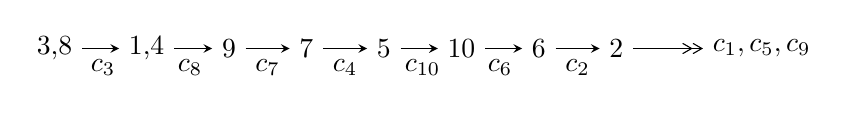
\begin{tikzpicture}[x=28pt, y=7pt]
	% node
	\node (A0) at (-1/8, 0) {3,8};
	\node (A1) at (17/16, 0) {1,4};
	\node (A2) at (17/8, 0) {9};
	\node (A3) at (25/8, 0) {7};
	\node (A4) at (33/8, 0) {5};
	\node (A5) at (41/8, 0) {10};
	\node (A6) at (49/8, 0) {6};
	\node (A7) at (57/8, 0) {2};
	\node (C1) at (1/2, -1) {$c_{3}$};
	\node (C2) at (13/8, -1) {$c_{8}$};
	\node (C3) at (21/8, -1) {$c_{7}$};
	\node (C4) at (29/8, -1) {$c_{4}$};
	\node (C5) at (37/8, -1) {$c_{10}$};
	\node (C6) at (45/8, -1) {$c_{6}$};
	\node (C7) at (53/8, -1) {$c_{2}$};
	\node (A8) at (9, 0) {$c_{1},c_{5},c_{9}$};

	% edge
	\draw[->,>=stealth]	
	(A0) edge (A1) (A1) edge (A2) (A2) edge (A3) (A3) edge (A4) (A4) edge (A5) (A5) edge (A6) (A6) edge (A7) ;
	\draw[->>,>={angle 60}]	
	(A7) edge (A8);
\end{tikzpicture} \\ 

\end{tabular} \\

\footnotetext{
The image of knot diagram is generated by the software ``\textbf{Draw programme}" developed by Andrew Bartholomew(\url{http://www.layer8.co.uk/maths/draw/index.htm\#Running-draw}), where we modified some parts for our purpose(\url{https://github.com/CATsTAILs/LinksPainter}).
}\phantom \\ \newline 
\centering \textbf{Ideals for irreducible components\footnotemark of $X_{\text{par}}$} 
 
\begin{align*}
I^u_{1}&=\langle 
149 u^{22}-622 u^{21}+\cdots+293 b-2738,\;-2738 u^{22}+12647 u^{21}+\cdots+2051 a+19961,\\
\phantom{I^u_{1}}&\phantom{= \langle  }u^{23}-5 u^{22}+\cdots-46 u+7\rangle \\
I^u_{2}&=\langle 
- u^{14}-3 u^{13}+\cdots+b+1,\;u^{14} a+u^{14}+\cdots- a-4,\\
\phantom{I^u_{2}}&\phantom{= \langle  }u^{15}+3 u^{14}+12 u^{13}+25 u^{12}+52 u^{11}+78 u^{10}+104 u^9+109 u^8+94 u^7+58 u^6+24 u^5-2 u^4-8 u^3-4 u^2+1\rangle \\
I^u_{3}&=\langle 
u^5+2 u^4+4 u^3+4 u^2+b+3 u+1,\;- u^7-2 u^6-6 u^5-7 u^4-9 u^3-5 u^2+a-3 u+1,\\
\phantom{I^u_{3}}&\phantom{= \langle  }u^8+2 u^7+6 u^6+8 u^5+11 u^4+9 u^3+7 u^2+2 u+1\rangle \\
\\
I^v_{1}&=\langle 
a,\;b+1,\;v-1\rangle \\
\end{align*}
\raggedright * 4 irreducible components of $\dim_{\mathbb{C}}=0$, with total 62 representations.\\
\footnotetext{All coefficients of polynomials are rational numbers. But the coefficients are sometimes approximated in decimal forms when there is not enough margin.}
\newpage
\renewcommand{\arraystretch}{1}
\centering \section*{I. $I^u_{1}= \langle 149 u^{22}-622 u^{21}+\cdots+293 b-2738,\;-2738 u^{22}+12647 u^{21}+\cdots+2051 a+19961,\;u^{23}-5 u^{22}+\cdots-46 u+7 \rangle$}
\flushleft \textbf{(i) Arc colorings}\\
\begin{tabular}{m{7pt} m{180pt} m{7pt} m{180pt} }
\flushright $a_{3}=$&$\begin{pmatrix}1\\0\end{pmatrix}$ \\
\flushright $a_{8}=$&$\begin{pmatrix}0\\u\end{pmatrix}$ \\
\flushright $a_{1}=$&$\begin{pmatrix}1.33496 u^{22}-6.16626 u^{21}+\cdots+74.2716 u-9.73233\\-0.508532 u^{22}+2.12287 u^{21}+\cdots-51.6758 u+9.34471\end{pmatrix}$ \\
\flushright $a_{4}=$&$\begin{pmatrix}1\\- u^2\end{pmatrix}$ \\
\flushright $a_{9}=$&$\begin{pmatrix}-3.13701 u^{22}+14.7157 u^{21}+\cdots-146.794 u+20.1351\\0.969283 u^{22}-4.75768 u^{21}+\cdots+125.167 u-21.9590\end{pmatrix}$ \\
\flushright $a_{7}=$&$\begin{pmatrix}- u\\u^3+u\end{pmatrix}$ \\
\flushright $a_{5}=$&$\begin{pmatrix}u^2+1\\- u^4-2 u^2\end{pmatrix}$ \\
\flushright $a_{10}=$&$\begin{pmatrix}0.826426 u^{22}-4.04339 u^{21}+\cdots+22.5958 u-0.387616\\-0.508532 u^{22}+2.12287 u^{21}+\cdots-51.6758 u+9.34471\end{pmatrix}$ \\
\flushright $a_{6}=$&$\begin{pmatrix}1.11555 u^{22}-4.72111 u^{21}+\cdots+61.6090 u-12.8684\\0.436860 u^{22}-0.890785 u^{21}+\cdots-12.6007 u+4.75085\end{pmatrix}$ \\
\flushright $a_{2}=$&$\begin{pmatrix}0.689907 u^{22}-3.07752 u^{21}+\cdots+27.7835 u-2.87226\\-0.136519 u^{22}+0.965870 u^{21}+\cdots-24.8123 u+3.51536\end{pmatrix}$\\&\end{tabular}
\flushleft \textbf{(ii) Obstruction class $= -1$}\\~\\
\flushleft \textbf{(iii) Cusp Shapes $= \frac{1041}{293} u^{22}-\frac{5380}{293} u^{21}+\cdots+\frac{116025}{293} u-\frac{22191}{293}$}\\~\\
\newpage\renewcommand{\arraystretch}{1}
\flushleft \textbf{(iv) u-Polynomials at the component}\newline \\
\begin{tabular}{m{50pt}|m{274pt}}
Crossings & \hspace{64pt}u-Polynomials at each crossing \\
\hline $$\begin{aligned}c_{1},c_{6}\end{aligned}$$&$\begin{aligned}
&u^{23}-2 u^{22}+\cdots-2 u-1
\end{aligned}$\\
\hline $$\begin{aligned}c_{2},c_{5}\end{aligned}$$&$\begin{aligned}
&u^{23}- u^{22}+\cdots- u-1
\end{aligned}$\\
\hline $$\begin{aligned}c_{3},c_{4},c_{7}\end{aligned}$$&$\begin{aligned}
&u^{23}+5 u^{22}+\cdots-46 u-7
\end{aligned}$\\
\hline $$\begin{aligned}c_{8},c_{10}\end{aligned}$$&$\begin{aligned}
&u^{23}+2 u^{22}+\cdots+14 u-1
\end{aligned}$\\
\hline $$\begin{aligned}c_{9}\end{aligned}$$&$\begin{aligned}
&u^{23}+14 u^{22}+\cdots-43 u-7
\end{aligned}$\\
\hline
\end{tabular}\\~\\
\newpage\renewcommand{\arraystretch}{1}
\flushleft \textbf{(v) Riley Polynomials at the component}\newline \\
\begin{tabular}{m{50pt}|m{274pt}}
Crossings & \hspace{64pt}Riley Polynomials at each crossing \\
\hline $$\begin{aligned}c_{1},c_{6}\end{aligned}$$&$\begin{aligned}
&y^{23}+2 y^{22}+\cdots-12 y-1
\end{aligned}$\\
\hline $$\begin{aligned}c_{2},c_{5}\end{aligned}$$&$\begin{aligned}
&y^{23}-9 y^{22}+\cdots+25 y-1
\end{aligned}$\\
\hline $$\begin{aligned}c_{3},c_{4},c_{7}\end{aligned}$$&$\begin{aligned}
&y^{23}+23 y^{22}+\cdots+198 y-49
\end{aligned}$\\
\hline $$\begin{aligned}c_{8},c_{10}\end{aligned}$$&$\begin{aligned}
&y^{23}-18 y^{22}+\cdots+68 y-1
\end{aligned}$\\
\hline $$\begin{aligned}c_{9}\end{aligned}$$&$\begin{aligned}
&y^{23}+26 y^{21}+\cdots+225 y-49
\end{aligned}$\\
\hline
\end{tabular}\\~\\
\newpage\flushleft \textbf{(vi) Complex Volumes and Cusp Shapes}
$$\begin{array}{c|c|c}  
\text{Solutions to }I^u_{1}& \I (\text{vol} + \sqrt{-1}CS) & \text{Cusp shape}\\
 \hline 
\begin{aligned}
u &= \phantom{-}0.746057 + 0.716204 I \\
a &= -0.944626 + 0.309140 I \\
b &= \phantom{-}0.926152 + 0.445909 I\end{aligned}
 & -1.41145 - 5.79407 I & -0.88331 + 5.20349 I \\ \hline\begin{aligned}
u &= \phantom{-}0.746057 - 0.716204 I \\
a &= -0.944626 - 0.309140 I \\
b &= \phantom{-}0.926152 - 0.445909 I\end{aligned}
 & -1.41145 + 5.79407 I & -0.88331 - 5.20349 I \\ \hline\begin{aligned}
u &= \phantom{-}0.838014 + 0.461206 I \\
a &= -0.68916 + 1.31806 I \\
b &= \phantom{-}1.18542 - 0.78671 I\end{aligned}
 & -0.67120 + 11.14210 I & \phantom{-}1.22299 - 8.55675 I \\ \hline\begin{aligned}
u &= \phantom{-}0.838014 - 0.461206 I \\
a &= -0.68916 - 1.31806 I \\
b &= \phantom{-}1.18542 + 0.78671 I\end{aligned}
 & -0.67120 - 11.14210 I & \phantom{-}1.22299 + 8.55675 I \\ \hline\begin{aligned}
u &= -0.638103 + 0.842766 I \\
a &= \phantom{-}0.134410 + 0.113744 I \\
b &= \phantom{-}0.181627 - 0.040696 I\end{aligned}
 & \phantom{-}0.67100 - 2.44356 I & \phantom{-}2.46207 - 5.34596 I \\ \hline\begin{aligned}
u &= -0.638103 - 0.842766 I \\
a &= \phantom{-}0.134410 - 0.113744 I \\
b &= \phantom{-}0.181627 + 0.040696 I\end{aligned}
 & \phantom{-}0.67100 + 2.44356 I & \phantom{-}2.46207 + 5.34596 I \\ \hline\begin{aligned}
u &= -0.134358 + 1.265940 I \\
a &= \phantom{-}0.552051 + 0.174175 I \\
b &= \phantom{-}0.294667 - 0.675459 I\end{aligned}
 & -2.55142 - 2.44221 I & \phantom{-}0.25016 + 2.15872 I \\ \hline\begin{aligned}
u &= -0.134358 - 1.265940 I \\
a &= \phantom{-}0.552051 - 0.174175 I \\
b &= \phantom{-}0.294667 + 0.675459 I\end{aligned}
 & -2.55142 + 2.44221 I & \phantom{-}0.25016 - 2.15872 I \\ \hline\begin{aligned}
u &= \phantom{-}0.571973 + 0.376783 I \\
a &= \phantom{-}0.67318 - 1.94063 I \\
b &= -1.116240 + 0.856342 I\end{aligned}
 & -1.92126 + 3.42239 I & -4.06899 - 7.96024 I \\ \hline\begin{aligned}
u &= \phantom{-}0.571973 - 0.376783 I \\
a &= \phantom{-}0.67318 + 1.94063 I \\
b &= -1.116240 - 0.856342 I\end{aligned}
 & -1.92126 - 3.42239 I & -4.06899 + 7.96024 I\\
 \hline 
 \end{array}$$\newpage$$\begin{array}{c|c|c}  
\text{Solutions to }I^u_{1}& \I (\text{vol} + \sqrt{-1}CS) & \text{Cusp shape}\\
 \hline 
\begin{aligned}
u &= -0.024762 + 1.413530 I \\
a &= -0.463614 - 0.845353 I \\
b &= -1.206410 + 0.634398 I\end{aligned}
 & -6.65304 - 0.20600 I & -5.87376 - 0.49624 I \\ \hline\begin{aligned}
u &= -0.024762 - 1.413530 I \\
a &= -0.463614 + 0.845353 I \\
b &= -1.206410 - 0.634398 I\end{aligned}
 & -6.65304 + 0.20600 I & -5.87376 + 0.49624 I \\ \hline\begin{aligned}
u &= \phantom{-}0.26611 + 1.40784 I \\
a &= \phantom{-}0.095717 - 0.962667 I \\
b &= -1.380760 + 0.121423 I\end{aligned}
 & -7.16412 + 2.89840 I & -6.40584 - 0.61240 I \\ \hline\begin{aligned}
u &= \phantom{-}0.26611 - 1.40784 I \\
a &= \phantom{-}0.095717 + 0.962667 I \\
b &= -1.380760 - 0.121423 I\end{aligned}
 & -7.16412 - 2.89840 I & -6.40584 + 0.61240 I \\ \hline\begin{aligned}
u &= -0.541870\phantom{ +0.000000I} \\
a &= \phantom{-}0.563072\phantom{ +0.000000I} \\
b &= \phantom{-}0.305112\phantom{ +0.000000I}\end{aligned}
 & \phantom{-}1.26878\phantom{ +0.000000I} & \phantom{-}7.95590\phantom{ +0.000000I} \\ \hline\begin{aligned}
u &= \phantom{-}0.476919 + 0.256901 I \\
a &= \phantom{-}1.77295 - 0.55054 I \\
b &= -0.986987 - 0.192913 I\end{aligned}
 & -1.97196 - 0.18097 I & -4.00287 - 0.43243 I \\ \hline\begin{aligned}
u &= \phantom{-}0.476919 - 0.256901 I \\
a &= \phantom{-}1.77295 + 0.55054 I \\
b &= -0.986987 + 0.192913 I\end{aligned}
 & -1.97196 + 0.18097 I & -4.00287 + 0.43243 I \\ \hline\begin{aligned}
u &= \phantom{-}0.21309 + 1.44798 I \\
a &= -0.594646 - 1.149250 I \\
b &= -1.53737 + 1.10594 I\end{aligned}
 & -7.80750 + 6.31614 I & -8.73055 - 7.98600 I \\ \hline\begin{aligned}
u &= \phantom{-}0.21309 - 1.44798 I \\
a &= -0.594646 + 1.149250 I \\
b &= -1.53737 - 1.10594 I\end{aligned}
 & -7.80750 - 6.31614 I & -8.73055 + 7.98600 I \\ \hline\begin{aligned}
u &= \phantom{-}0.30585 + 1.51255 I \\
a &= \phantom{-}0.399853 + 1.070490 I \\
b &= \phantom{-}1.49687 - 0.93220 I\end{aligned}
 & -7.0586 + 15.3049 I & -1.91417 - 8.23545 I\\
 \hline 
 \end{array}$$\newpage$$\begin{array}{c|c|c}  
\text{Solutions to }I^u_{1}& \I (\text{vol} + \sqrt{-1}CS) & \text{Cusp shape}\\
 \hline 
\begin{aligned}
u &= \phantom{-}0.30585 - 1.51255 I \\
a &= \phantom{-}0.399853 - 1.070490 I \\
b &= \phantom{-}1.49687 + 0.93220 I\end{aligned}
 & -7.0586 - 15.3049 I & -1.91417 + 8.23545 I \\ \hline\begin{aligned}
u &= \phantom{-}0.15014 + 1.58348 I \\
a &= \phantom{-}0.068059 + 0.631954 I \\
b &= \phantom{-}0.990467 - 0.202654 I\end{aligned}
 & -9.33057 - 2.66158 I & -5.53368 + 3.29637 I \\ \hline\begin{aligned}
u &= \phantom{-}0.15014 - 1.58348 I \\
a &= \phantom{-}0.068059 - 0.631954 I \\
b &= \phantom{-}0.990467 + 0.202654 I\end{aligned}
 & -9.33057 + 2.66158 I & -5.53368 - 3.29637 I\\
 \hline 
 \end{array}$$\newpage\newpage\renewcommand{\arraystretch}{1}
\centering \section*{II. $I^u_{2}= \langle - u^{14}-3 u^{13}+\cdots+b+1,\;u^{14} a+u^{14}+\cdots- a-4,\;u^{15}+3 u^{14}+\cdots-4 u^2+1 \rangle$}
\flushleft \textbf{(i) Arc colorings}\\
\begin{tabular}{m{7pt} m{180pt} m{7pt} m{180pt} }
\flushright $a_{3}=$&$\begin{pmatrix}1\\0\end{pmatrix}$ \\
\flushright $a_{8}=$&$\begin{pmatrix}0\\u\end{pmatrix}$ \\
\flushright $a_{1}=$&$\begin{pmatrix}a\\u^{14}+3 u^{13}+\cdots- u-1\end{pmatrix}$ \\
\flushright $a_{4}=$&$\begin{pmatrix}1\\- u^2\end{pmatrix}$ \\
\flushright $a_{9}=$&$\begin{pmatrix}u^{14} a+u^{14}+\cdots- a-1\\-1\end{pmatrix}$ \\
\flushright $a_{7}=$&$\begin{pmatrix}- u\\u^3+u\end{pmatrix}$ \\
\flushright $a_{5}=$&$\begin{pmatrix}u^2+1\\- u^4-2 u^2\end{pmatrix}$ \\
\flushright $a_{10}=$&$\begin{pmatrix}u^{14}+3 u^{13}+\cdots+a-1\\u^{14}+3 u^{13}+\cdots- u-1\end{pmatrix}$ \\
\flushright $a_{6}=$&$\begin{pmatrix}u^{14}+3 u^{13}+\cdots- a-2\\- u^{12} a-3 u^{11} a+\cdots+2 u+1\end{pmatrix}$ \\
\flushright $a_{2}=$&$\begin{pmatrix}u^{14}+3 u^{13}+\cdots+a-1\\- u^8 a+u^8+\cdots+a u-1\end{pmatrix}$\\&\end{tabular}
\flushleft \textbf{(ii) Obstruction class $= -1$}\\~\\
\flushleft \textbf{(iii) Cusp Shapes $= 4 u^{14}+4 u^{13}+24 u^{12}+12 u^{11}+32 u^{10}-24 u^9-56 u^8-136 u^7-172 u^6-184 u^5-124 u^4-72 u^3-8 u^2+16 u+10$}\\~\\
\newpage\renewcommand{\arraystretch}{1}
\flushleft \textbf{(iv) u-Polynomials at the component}\newline \\
\begin{tabular}{m{50pt}|m{274pt}}
Crossings & \hspace{64pt}u-Polynomials at each crossing \\
\hline $$\begin{aligned}c_{1},c_{6}\end{aligned}$$&$\begin{aligned}
&u^{30}+u^{29}+\cdots+16 u+1
\end{aligned}$\\
\hline $$\begin{aligned}c_{2},c_{5}\end{aligned}$$&$\begin{aligned}
&u^{30}+u^{29}+\cdots-6 u-1
\end{aligned}$\\
\hline $$\begin{aligned}c_{3},c_{4},c_{7}\end{aligned}$$&$\begin{aligned}
&(u^{15}-3 u^{14}+\cdots+4 u^2-1)^{2}
\end{aligned}$\\
\hline $$\begin{aligned}c_{8},c_{10}\end{aligned}$$&$\begin{aligned}
&u^{30}- u^{29}+\cdots-6 u-11
\end{aligned}$\\
\hline $$\begin{aligned}c_{9}\end{aligned}$$&$\begin{aligned}
&(u^{15}-7 u^{14}+\cdots+4 u^2-1)^{2}
\end{aligned}$\\
\hline
\end{tabular}\\~\\
\newpage\renewcommand{\arraystretch}{1}
\flushleft \textbf{(v) Riley Polynomials at the component}\newline \\
\begin{tabular}{m{50pt}|m{274pt}}
Crossings & \hspace{64pt}Riley Polynomials at each crossing \\
\hline $$\begin{aligned}c_{1},c_{6}\end{aligned}$$&$\begin{aligned}
&y^{30}+3 y^{29}+\cdots-92 y+1
\end{aligned}$\\
\hline $$\begin{aligned}c_{2},c_{5}\end{aligned}$$&$\begin{aligned}
&y^{30}+7 y^{29}+\cdots-48 y+1
\end{aligned}$\\
\hline $$\begin{aligned}c_{3},c_{4},c_{7}\end{aligned}$$&$\begin{aligned}
&(y^{15}+15 y^{14}+\cdots+8 y-1)^{2}
\end{aligned}$\\
\hline $$\begin{aligned}c_{8},c_{10}\end{aligned}$$&$\begin{aligned}
&y^{30}+3 y^{29}+\cdots-1972 y+121
\end{aligned}$\\
\hline $$\begin{aligned}c_{9}\end{aligned}$$&$\begin{aligned}
&(y^{15}- y^{14}+\cdots+8 y-1)^{2}
\end{aligned}$\\
\hline
\end{tabular}\\~\\
\newpage\flushleft \textbf{(vi) Complex Volumes and Cusp Shapes}
$$\begin{array}{c|c|c}  
\text{Solutions to }I^u_{2}& \I (\text{vol} + \sqrt{-1}CS) & \text{Cusp shape}\\
 \hline 
\begin{aligned}
u &= -0.825834 + 0.538674 I \\
a &= \phantom{-}0.428447 + 0.718077 I \\
b &= -0.476814 - 0.494120 I\end{aligned}
 & \phantom{-}1.13071 - 2.72262 I & \phantom{-}11.6934 + 8.2204 I \\ \hline\begin{aligned}
u &= -0.825834 + 0.538674 I \\
a &= -0.131251 - 0.683941 I \\
b &= \phantom{-}0.740636 + 0.362219 I\end{aligned}
 & \phantom{-}1.13071 - 2.72262 I & \phantom{-}11.6934 + 8.2204 I \\ \hline\begin{aligned}
u &= -0.825834 - 0.538674 I \\
a &= \phantom{-}0.428447 - 0.718077 I \\
b &= -0.476814 + 0.494120 I\end{aligned}
 & \phantom{-}1.13071 + 2.72262 I & \phantom{-}11.6934 - 8.2204 I \\ \hline\begin{aligned}
u &= -0.825834 - 0.538674 I \\
a &= -0.131251 + 0.683941 I \\
b &= \phantom{-}0.740636 - 0.362219 I\end{aligned}
 & \phantom{-}1.13071 + 2.72262 I & \phantom{-}11.6934 - 8.2204 I \\ \hline\begin{aligned}
u &= \phantom{-}0.000696 + 1.255430 I \\
a &= \phantom{-}0.900707 - 0.205837 I \\
b &= \phantom{-}1.247670 - 0.599225 I\end{aligned}
 & -1.82383 - 2.53738 I & \phantom{-}2.44510 + 1.72215 I \\ \hline\begin{aligned}
u &= \phantom{-}0.000696 + 1.255430 I \\
a &= \phantom{-}0.476757 + 0.994088 I \\
b &= -0.259040 - 1.130630 I\end{aligned}
 & -1.82383 - 2.53738 I & \phantom{-}2.44510 + 1.72215 I \\ \hline\begin{aligned}
u &= \phantom{-}0.000696 - 1.255430 I \\
a &= \phantom{-}0.900707 + 0.205837 I \\
b &= \phantom{-}1.247670 + 0.599225 I\end{aligned}
 & -1.82383 + 2.53738 I & \phantom{-}2.44510 - 1.72215 I \\ \hline\begin{aligned}
u &= \phantom{-}0.000696 - 1.255430 I \\
a &= \phantom{-}0.476757 - 0.994088 I \\
b &= -0.259040 + 1.130630 I\end{aligned}
 & -1.82383 + 2.53738 I & \phantom{-}2.44510 - 1.72215 I \\ \hline\begin{aligned}
u &= -0.374558 + 0.641779 I \\
a &= \phantom{-}0.471003 + 0.871968 I \\
b &= -0.877609 - 0.842947 I\end{aligned}
 & -1.31377 - 3.39671 I & -3.52800 + 8.19673 I \\ \hline\begin{aligned}
u &= -0.374558 + 0.641779 I \\
a &= \phantom{-}0.38443 - 1.59182 I \\
b &= \phantom{-}0.736028 + 0.024323 I\end{aligned}
 & -1.31377 - 3.39671 I & -3.52800 + 8.19673 I\\
 \hline 
 \end{array}$$\newpage$$\begin{array}{c|c|c}  
\text{Solutions to }I^u_{2}& \I (\text{vol} + \sqrt{-1}CS) & \text{Cusp shape}\\
 \hline 
\begin{aligned}
u &= -0.374558 - 0.641779 I \\
a &= \phantom{-}0.471003 - 0.871968 I \\
b &= -0.877609 + 0.842947 I\end{aligned}
 & -1.31377 + 3.39671 I & -3.52800 - 8.19673 I \\ \hline\begin{aligned}
u &= -0.374558 - 0.641779 I \\
a &= \phantom{-}0.38443 + 1.59182 I \\
b &= \phantom{-}0.736028 - 0.024323 I\end{aligned}
 & -1.31377 + 3.39671 I & -3.52800 - 8.19673 I \\ \hline\begin{aligned}
u &= -0.678314\phantom{ +0.000000I} \\
a &= \phantom{-}1.44772\phantom{ +0.000000I} \\
b &= -0.327578\phantom{ +0.000000I}\end{aligned}
 & \phantom{-}1.01641\phantom{ +0.000000I} & \phantom{-}9.27190\phantom{ +0.000000I} \\ \hline\begin{aligned}
u &= -0.678314\phantom{ +0.000000I} \\
a &= -0.482930\phantom{ +0.000000I} \\
b &= \phantom{-}0.982011\phantom{ +0.000000I}\end{aligned}
 & \phantom{-}1.01641\phantom{ +0.000000I} & \phantom{-}9.27190\phantom{ +0.000000I} \\ \hline\begin{aligned}
u &= \phantom{-}0.100337 + 1.375660 I \\
a &= -0.268106 - 0.521008 I \\
b &= \phantom{-}0.27520 + 2.16220 I\end{aligned}
 & -3.32174 + 5.59550 I & -0.66951 - 7.79345 I \\ \hline\begin{aligned}
u &= \phantom{-}0.100337 + 1.375660 I \\
a &= -1.57796 + 0.08496 I \\
b &= -0.689826 + 0.421097 I\end{aligned}
 & -3.32174 + 5.59550 I & -0.66951 - 7.79345 I \\ \hline\begin{aligned}
u &= \phantom{-}0.100337 - 1.375660 I \\
a &= -0.268106 + 0.521008 I \\
b &= \phantom{-}0.27520 - 2.16220 I\end{aligned}
 & -3.32174 - 5.59550 I & -0.66951 + 7.79345 I \\ \hline\begin{aligned}
u &= \phantom{-}0.100337 - 1.375660 I \\
a &= -1.57796 - 0.08496 I \\
b &= -0.689826 - 0.421097 I\end{aligned}
 & -3.32174 - 5.59550 I & -0.66951 + 7.79345 I \\ \hline\begin{aligned}
u &= -0.15235 + 1.51729 I \\
a &= \phantom{-}0.516022 - 1.130560 I \\
b &= \phantom{-}0.789858 + 0.466052 I\end{aligned}
 & -8.32063 - 5.47678 I & -8.29813 + 5.38780 I \\ \hline\begin{aligned}
u &= -0.15235 + 1.51729 I \\
a &= -0.252346 + 0.545908 I \\
b &= -1.63678 - 0.95520 I\end{aligned}
 & -8.32063 - 5.47678 I & -8.29813 + 5.38780 I\\
 \hline 
 \end{array}$$\newpage$$\begin{array}{c|c|c}  
\text{Solutions to }I^u_{2}& \I (\text{vol} + \sqrt{-1}CS) & \text{Cusp shape}\\
 \hline 
\begin{aligned}
u &= -0.15235 - 1.51729 I \\
a &= \phantom{-}0.516022 + 1.130560 I \\
b &= \phantom{-}0.789858 - 0.466052 I\end{aligned}
 & -8.32063 + 5.47678 I & -8.29813 - 5.38780 I \\ \hline\begin{aligned}
u &= -0.15235 - 1.51729 I \\
a &= -0.252346 - 0.545908 I \\
b &= -1.63678 + 0.95520 I\end{aligned}
 & -8.32063 + 5.47678 I & -8.29813 - 5.38780 I \\ \hline\begin{aligned}
u &= -0.29798 + 1.53037 I \\
a &= \phantom{-}0.439615 - 0.718620 I \\
b &= \phantom{-}1.181030 + 0.498484 I\end{aligned}
 & -5.55973 - 6.84757 I & \phantom{-}1.00546 + 10.27446 I \\ \hline\begin{aligned}
u &= -0.29798 + 1.53037 I \\
a &= -0.169055 + 0.804639 I \\
b &= -0.968761 - 0.886910 I\end{aligned}
 & -5.55973 - 6.84757 I & \phantom{-}1.00546 + 10.27446 I \\ \hline\begin{aligned}
u &= -0.29798 - 1.53037 I \\
a &= \phantom{-}0.439615 + 0.718620 I \\
b &= \phantom{-}1.181030 - 0.498484 I\end{aligned}
 & -5.55973 + 6.84757 I & \phantom{-}1.00546 - 10.27446 I \\ \hline\begin{aligned}
u &= -0.29798 - 1.53037 I \\
a &= -0.169055 - 0.804639 I \\
b &= -0.968761 + 0.886910 I\end{aligned}
 & -5.55973 + 6.84757 I & \phantom{-}1.00546 - 10.27446 I \\ \hline\begin{aligned}
u &= \phantom{-}0.388845 + 0.104061 I \\
a &= \phantom{-}0.40559 - 2.33647 I \\
b &= \phantom{-}0.51204 + 1.36623 I\end{aligned}
 & \phantom{-}1.42898 + 3.92960 I & \phantom{-}9.71569 - 7.98755 I \\ \hline\begin{aligned}
u &= \phantom{-}0.388845 + 0.104061 I \\
a &= -2.10625 - 2.94990 I \\
b &= -0.400846 + 0.866321 I\end{aligned}
 & \phantom{-}1.42898 + 3.92960 I & \phantom{-}9.71569 - 7.98755 I \\ \hline\begin{aligned}
u &= \phantom{-}0.388845 - 0.104061 I \\
a &= \phantom{-}0.40559 + 2.33647 I \\
b &= \phantom{-}0.51204 - 1.36623 I\end{aligned}
 & \phantom{-}1.42898 - 3.92960 I & \phantom{-}9.71569 + 7.98755 I \\ \hline\begin{aligned}
u &= \phantom{-}0.388845 - 0.104061 I \\
a &= -2.10625 + 2.94990 I \\
b &= -0.400846 - 0.866321 I\end{aligned}
 & \phantom{-}1.42898 - 3.92960 I & \phantom{-}9.71569 + 7.98755 I\\
 \hline 
 \end{array}$$\newpage\newpage\renewcommand{\arraystretch}{1}
\centering \section*{III. $I^u_{3}= \langle u^5+2 u^4+4 u^3+4 u^2+b+3 u+1,\;- u^7-2 u^6+\cdots+a+1,\;u^8+2 u^7+\cdots+2 u+1 \rangle$}
\flushleft \textbf{(i) Arc colorings}\\
\begin{tabular}{m{7pt} m{180pt} m{7pt} m{180pt} }
\flushright $a_{3}=$&$\begin{pmatrix}1\\0\end{pmatrix}$ \\
\flushright $a_{8}=$&$\begin{pmatrix}0\\u\end{pmatrix}$ \\
\flushright $a_{1}=$&$\begin{pmatrix}u^7+2 u^6+6 u^5+7 u^4+9 u^3+5 u^2+3 u-1\\- u^5-2 u^4-4 u^3-4 u^2-3 u-1\end{pmatrix}$ \\
\flushright $a_{4}=$&$\begin{pmatrix}1\\- u^2\end{pmatrix}$ \\
\flushright $a_{9}=$&$\begin{pmatrix}- u^7-2 u^6-5 u^5-7 u^4-8 u^3-7 u^2-5 u-2\\u^6+u^5+3 u^4+2 u^3+2 u^2+u+1\end{pmatrix}$ \\
\flushright $a_{7}=$&$\begin{pmatrix}- u\\u^3+u\end{pmatrix}$ \\
\flushright $a_{5}=$&$\begin{pmatrix}u^2+1\\- u^4-2 u^2\end{pmatrix}$ \\
\flushright $a_{10}=$&$\begin{pmatrix}u^7+2 u^6+5 u^5+5 u^4+5 u^3+u^2-2\\- u^5-2 u^4-4 u^3-4 u^2-3 u-1\end{pmatrix}$ \\
\flushright $a_{6}=$&$\begin{pmatrix}- u^7-2 u^6-6 u^5-8 u^4-11 u^3-8 u^2-6 u\\u^3+u^2+2 u+1\end{pmatrix}$ \\
\flushright $a_{2}=$&$\begin{pmatrix}u^7+2 u^6+5 u^5+6 u^4+6 u^3+3 u^2+u-1\\- u^6-2 u^5-5 u^4-6 u^3-6 u^2-4 u-1\end{pmatrix}$\\&\end{tabular}
\flushleft \textbf{(ii) Obstruction class $= 1$}\\~\\
\flushleft \textbf{(iii) Cusp Shapes $= -3 u^7- u^6-3 u^5+8 u^4+17 u^3+19 u^2+18 u+5$}\\~\\
\newpage\renewcommand{\arraystretch}{1}
\flushleft \textbf{(iv) u-Polynomials at the component}\newline \\
\begin{tabular}{m{50pt}|m{274pt}}
Crossings & \hspace{64pt}u-Polynomials at each crossing \\
\hline $$\begin{aligned}c_{1},c_{6}\end{aligned}$$&$\begin{aligned}
&u^8- u^7+2 u^6- u^5+2 u^4- u^3+2 u^2+1
\end{aligned}$\\
\hline $$\begin{aligned}c_{2},c_{5}\end{aligned}$$&$\begin{aligned}
&u^8+2 u^6+u^5+2 u^4+u^3+2 u^2+u+1
\end{aligned}$\\
\hline $$\begin{aligned}c_{3},c_{4}\end{aligned}$$&$\begin{aligned}
&u^8+2 u^7+6 u^6+8 u^5+11 u^4+9 u^3+7 u^2+2 u+1
\end{aligned}$\\
\hline $$\begin{aligned}c_{7}\end{aligned}$$&$\begin{aligned}
&u^8-2 u^7+6 u^6-8 u^5+11 u^4-9 u^3+7 u^2-2 u+1
\end{aligned}$\\
\hline $$\begin{aligned}c_{8},c_{10}\end{aligned}$$&$\begin{aligned}
&u^8-3 u^7+6 u^6-9 u^5+12 u^4-11 u^3+8 u^2-4 u+1
\end{aligned}$\\
\hline $$\begin{aligned}c_{9}\end{aligned}$$&$\begin{aligned}
&u^8+5 u^7+13 u^6+20 u^5+22 u^4+18 u^3+12 u^2+5 u+1
\end{aligned}$\\
\hline
\end{tabular}\\~\\
\newpage\renewcommand{\arraystretch}{1}
\flushleft \textbf{(v) Riley Polynomials at the component}\newline \\
\begin{tabular}{m{50pt}|m{274pt}}
Crossings & \hspace{64pt}Riley Polynomials at each crossing \\
\hline $$\begin{aligned}c_{1},c_{6}\end{aligned}$$&$\begin{aligned}
&y^8+3 y^7+6 y^6+9 y^5+12 y^4+11 y^3+8 y^2+4 y+1
\end{aligned}$\\
\hline $$\begin{aligned}c_{2},c_{5}\end{aligned}$$&$\begin{aligned}
&y^8+4 y^7+8 y^6+11 y^5+12 y^4+9 y^3+6 y^2+3 y+1
\end{aligned}$\\
\hline $$\begin{aligned}c_{3},c_{4},c_{7}\end{aligned}$$&$\begin{aligned}
&y^8+8 y^7+26 y^6+46 y^5+55 y^4+53 y^3+35 y^2+10 y+1
\end{aligned}$\\
\hline $$\begin{aligned}c_{8},c_{10}\end{aligned}$$&$\begin{aligned}
&y^8+3 y^7+6 y^6+13 y^5+20 y^4+11 y^3+1
\end{aligned}$\\
\hline $$\begin{aligned}c_{9}\end{aligned}$$&$\begin{aligned}
&y^8+y^7+13 y^6+16 y^5+28 y^4+30 y^3+8 y^2- y+1
\end{aligned}$\\
\hline
\end{tabular}\\~\\
\newpage\flushleft \textbf{(vi) Complex Volumes and Cusp Shapes}
$$\begin{array}{c|c|c}  
\text{Solutions to }I^u_{3}& \I (\text{vol} + \sqrt{-1}CS) & \text{Cusp shape}\\
 \hline 
\begin{aligned}
u &= -0.768546 + 0.720795 I \\
a &= \phantom{-}0.216551 + 0.549851 I \\
b &= -0.562759 - 0.266496 I\end{aligned}
 & \phantom{-}0.48271 - 2.83701 I & -5.21159 + 10.60912 I \\ \hline\begin{aligned}
u &= -0.768546 - 0.720795 I \\
a &= \phantom{-}0.216551 - 0.549851 I \\
b &= -0.562759 + 0.266496 I\end{aligned}
 & \phantom{-}0.48271 + 2.83701 I & -5.21159 - 10.60912 I \\ \hline\begin{aligned}
u &= \phantom{-}0.024235 + 1.274500 I \\
a &= \phantom{-}0.986575 - 0.224172 I \\
b &= \phantom{-}0.309617 + 1.251960 I\end{aligned}
 & -2.47121 + 3.78237 I & -0.87896 - 6.92362 I \\ \hline\begin{aligned}
u &= \phantom{-}0.024235 - 1.274500 I \\
a &= \phantom{-}0.986575 + 0.224172 I \\
b &= \phantom{-}0.309617 - 1.251960 I\end{aligned}
 & -2.47121 - 3.78237 I & -0.87896 + 6.92362 I \\ \hline\begin{aligned}
u &= -0.057100 + 0.488588 I \\
a &= -1.72754 + 0.48541 I \\
b &= -0.138522 - 0.871772 I\end{aligned}
 & \phantom{-}0.43885 - 3.70343 I & \phantom{-}0.65225 + 5.99436 I \\ \hline\begin{aligned}
u &= -0.057100 - 0.488588 I \\
a &= -1.72754 - 0.48541 I \\
b &= -0.138522 + 0.871772 I\end{aligned}
 & \phantom{-}0.43885 + 3.70343 I & \phantom{-}0.65225 - 5.99436 I \\ \hline\begin{aligned}
u &= -0.19859 + 1.50044 I \\
a &= -0.475588 + 0.801618 I \\
b &= -1.108340 - 0.872786 I\end{aligned}
 & -6.67501 - 5.79166 I & -2.06170 + 5.06823 I \\ \hline\begin{aligned}
u &= -0.19859 - 1.50044 I \\
a &= -0.475588 - 0.801618 I \\
b &= -1.108340 + 0.872786 I\end{aligned}
 & -6.67501 + 5.79166 I & -2.06170 - 5.06823 I\\
 \hline 
 \end{array}$$\newpage\newpage\renewcommand{\arraystretch}{1}
\centering \section*{IV. $I^v_{1}= \langle a,\;b+1,\;v-1 \rangle$}
\flushleft \textbf{(i) Arc colorings}\\
\begin{tabular}{m{7pt} m{180pt} m{7pt} m{180pt} }
\flushright $a_{3}=$&$\begin{pmatrix}1\\0\end{pmatrix}$ \\
\flushright $a_{8}=$&$\begin{pmatrix}1\\0\end{pmatrix}$ \\
\flushright $a_{1}=$&$\begin{pmatrix}0\\-1\end{pmatrix}$ \\
\flushright $a_{4}=$&$\begin{pmatrix}1\\0\end{pmatrix}$ \\
\flushright $a_{9}=$&$\begin{pmatrix}1\\1\end{pmatrix}$ \\
\flushright $a_{7}=$&$\begin{pmatrix}1\\0\end{pmatrix}$ \\
\flushright $a_{5}=$&$\begin{pmatrix}1\\0\end{pmatrix}$ \\
\flushright $a_{10}=$&$\begin{pmatrix}-1\\-1\end{pmatrix}$ \\
\flushright $a_{6}=$&$\begin{pmatrix}2\\1\end{pmatrix}$ \\
\flushright $a_{2}=$&$\begin{pmatrix}-1\\-1\end{pmatrix}$\\&\end{tabular}
\flushleft \textbf{(ii) Obstruction class $= -1$}\\~\\
\flushleft \textbf{(iii) Cusp Shapes $= -6$}\\~\\
\newpage\renewcommand{\arraystretch}{1}
\flushleft \textbf{(iv) u-Polynomials at the component}\newline \\
\begin{tabular}{m{50pt}|m{274pt}}
Crossings & \hspace{64pt}u-Polynomials at each crossing \\
\hline $$\begin{aligned}c_{1},c_{2},c_{5}\\c_{6},c_{8},c_{10}\end{aligned}$$&$\begin{aligned}
&u+1
\end{aligned}$\\
\hline $$\begin{aligned}c_{3},c_{4},c_{7}\\c_{9}\end{aligned}$$&$\begin{aligned}
&u
\end{aligned}$\\
\hline
\end{tabular}\\~\\
\newpage\renewcommand{\arraystretch}{1}
\flushleft \textbf{(v) Riley Polynomials at the component}\newline \\
\begin{tabular}{m{50pt}|m{274pt}}
Crossings & \hspace{64pt}Riley Polynomials at each crossing \\
\hline $$\begin{aligned}c_{1},c_{2},c_{5}\\c_{6},c_{8},c_{10}\end{aligned}$$&$\begin{aligned}
&y-1
\end{aligned}$\\
\hline $$\begin{aligned}c_{3},c_{4},c_{7}\\c_{9}\end{aligned}$$&$\begin{aligned}
&y
\end{aligned}$\\
\hline
\end{tabular}\\~\\
\newpage\flushleft \textbf{(vi) Complex Volumes and Cusp Shapes}
$$\begin{array}{c|c|c}  
\text{Solutions to }I^v_{1}& \I (\text{vol} + \sqrt{-1}CS) & \text{Cusp shape}\\
 \hline 
\begin{aligned}
v &= \phantom{-}1.00000\phantom{ +0.000000I} \\
a &= \phantom{-0.000000 } 0 \\
b &= -1.00000\phantom{ +0.000000I}\end{aligned}
 & -1.64493\phantom{ +0.000000I} & -6.00000\phantom{ +0.000000I}\\
 \hline 
 \end{array}$$\newpage
\newpage\renewcommand{\arraystretch}{1}
\centering \section*{ V. u-Polynomials}
\begin{tabular}{m{50pt}|m{274pt}}
Crossings & \hspace{64pt}u-Polynomials at each crossing \\
\hline $$\begin{aligned}c_{1},c_{6}\end{aligned}$$&$\begin{aligned}
&(u+1)(u^8- u^7+\cdots+2 u^2+1)(u^{23}-2 u^{22}+\cdots-2 u-1)\\
&\cdot(u^{30}+u^{29}+\cdots+16 u+1)
\end{aligned}$\\
\hline $$\begin{aligned}c_{2},c_{5}\end{aligned}$$&$\begin{aligned}
&(u+1)(u^8+2 u^6+\cdots+u+1)(u^{23}- u^{22}+\cdots- u-1)\\
&\cdot(u^{30}+u^{29}+\cdots-6 u-1)
\end{aligned}$\\
\hline $$\begin{aligned}c_{3},c_{4}\end{aligned}$$&$\begin{aligned}
&u(u^8+2 u^7+6 u^6+8 u^5+11 u^4+9 u^3+7 u^2+2 u+1)\\
&\cdot((u^{15}-3 u^{14}+\cdots+4 u^2-1)^{2})(u^{23}+5 u^{22}+\cdots-46 u-7)
\end{aligned}$\\
\hline $$\begin{aligned}c_{7}\end{aligned}$$&$\begin{aligned}
&u(u^8-2 u^7+6 u^6-8 u^5+11 u^4-9 u^3+7 u^2-2 u+1)\\
&\cdot((u^{15}-3 u^{14}+\cdots+4 u^2-1)^{2})(u^{23}+5 u^{22}+\cdots-46 u-7)
\end{aligned}$\\
\hline $$\begin{aligned}c_{8},c_{10}\end{aligned}$$&$\begin{aligned}
&(u+1)(u^8-3 u^7+6 u^6-9 u^5+12 u^4-11 u^3+8 u^2-4 u+1)\\
&\cdot(u^{23}+2 u^{22}+\cdots+14 u-1)(u^{30}- u^{29}+\cdots-6 u-11)
\end{aligned}$\\
\hline $$\begin{aligned}c_{9}\end{aligned}$$&$\begin{aligned}
&u(u^8+5 u^7+13 u^6+20 u^5+22 u^4+18 u^3+12 u^2+5 u+1)\\
&\cdot((u^{15}-7 u^{14}+\cdots+4 u^2-1)^{2})(u^{23}+14 u^{22}+\cdots-43 u-7)
\end{aligned}$\\
\hline
\end{tabular}\newpage\renewcommand{\arraystretch}{1}
\centering \section*{ VI. Riley Polynomials}
\begin{tabular}{m{50pt}|m{274pt}}
Crossings & \hspace{64pt}Riley Polynomials at each crossing \\
\hline $$\begin{aligned}c_{1},c_{6}\end{aligned}$$&$\begin{aligned}
&(y-1)(y^8+3 y^7+6 y^6+9 y^5+12 y^4+11 y^3+8 y^2+4 y+1)\\
&\cdot(y^{23}+2 y^{22}+\cdots-12 y-1)(y^{30}+3 y^{29}+\cdots-92 y+1)
\end{aligned}$\\
\hline $$\begin{aligned}c_{2},c_{5}\end{aligned}$$&$\begin{aligned}
&(y-1)(y^8+4 y^7+8 y^6+11 y^5+12 y^4+9 y^3+6 y^2+3 y+1)\\
&\cdot(y^{23}-9 y^{22}+\cdots+25 y-1)(y^{30}+7 y^{29}+\cdots-48 y+1)
\end{aligned}$\\
\hline $$\begin{aligned}c_{3},c_{4},c_{7}\end{aligned}$$&$\begin{aligned}
&y(y^8+8 y^7+26 y^6+46 y^5+55 y^4+53 y^3+35 y^2+10 y+1)\\
&\cdot((y^{15}+15 y^{14}+\cdots+8 y-1)^{2})(y^{23}+23 y^{22}+\cdots+198 y-49)
\end{aligned}$\\
\hline $$\begin{aligned}c_{8},c_{10}\end{aligned}$$&$\begin{aligned}
&(y-1)(y^8+3 y^7+6 y^6+13 y^5+20 y^4+11 y^3+1)\\
&\cdot(y^{23}-18 y^{22}+\cdots+68 y-1)(y^{30}+3 y^{29}+\cdots-1972 y+121)
\end{aligned}$\\
\hline $$\begin{aligned}c_{9}\end{aligned}$$&$\begin{aligned}
&y(y^8+y^7+13 y^6+16 y^5+28 y^4+30 y^3+8 y^2- y+1)\\
&\cdot((y^{15}- y^{14}+\cdots+8 y-1)^{2})(y^{23}+26 y^{21}+\cdots+225 y-49)
\end{aligned}$\\
\hline
\end{tabular}
\vskip 2pc
\end{document}